\chapter{The Berkeley Analog Generator}

\section{Overview and Top Level}
\begin{figure}[h]
\centering
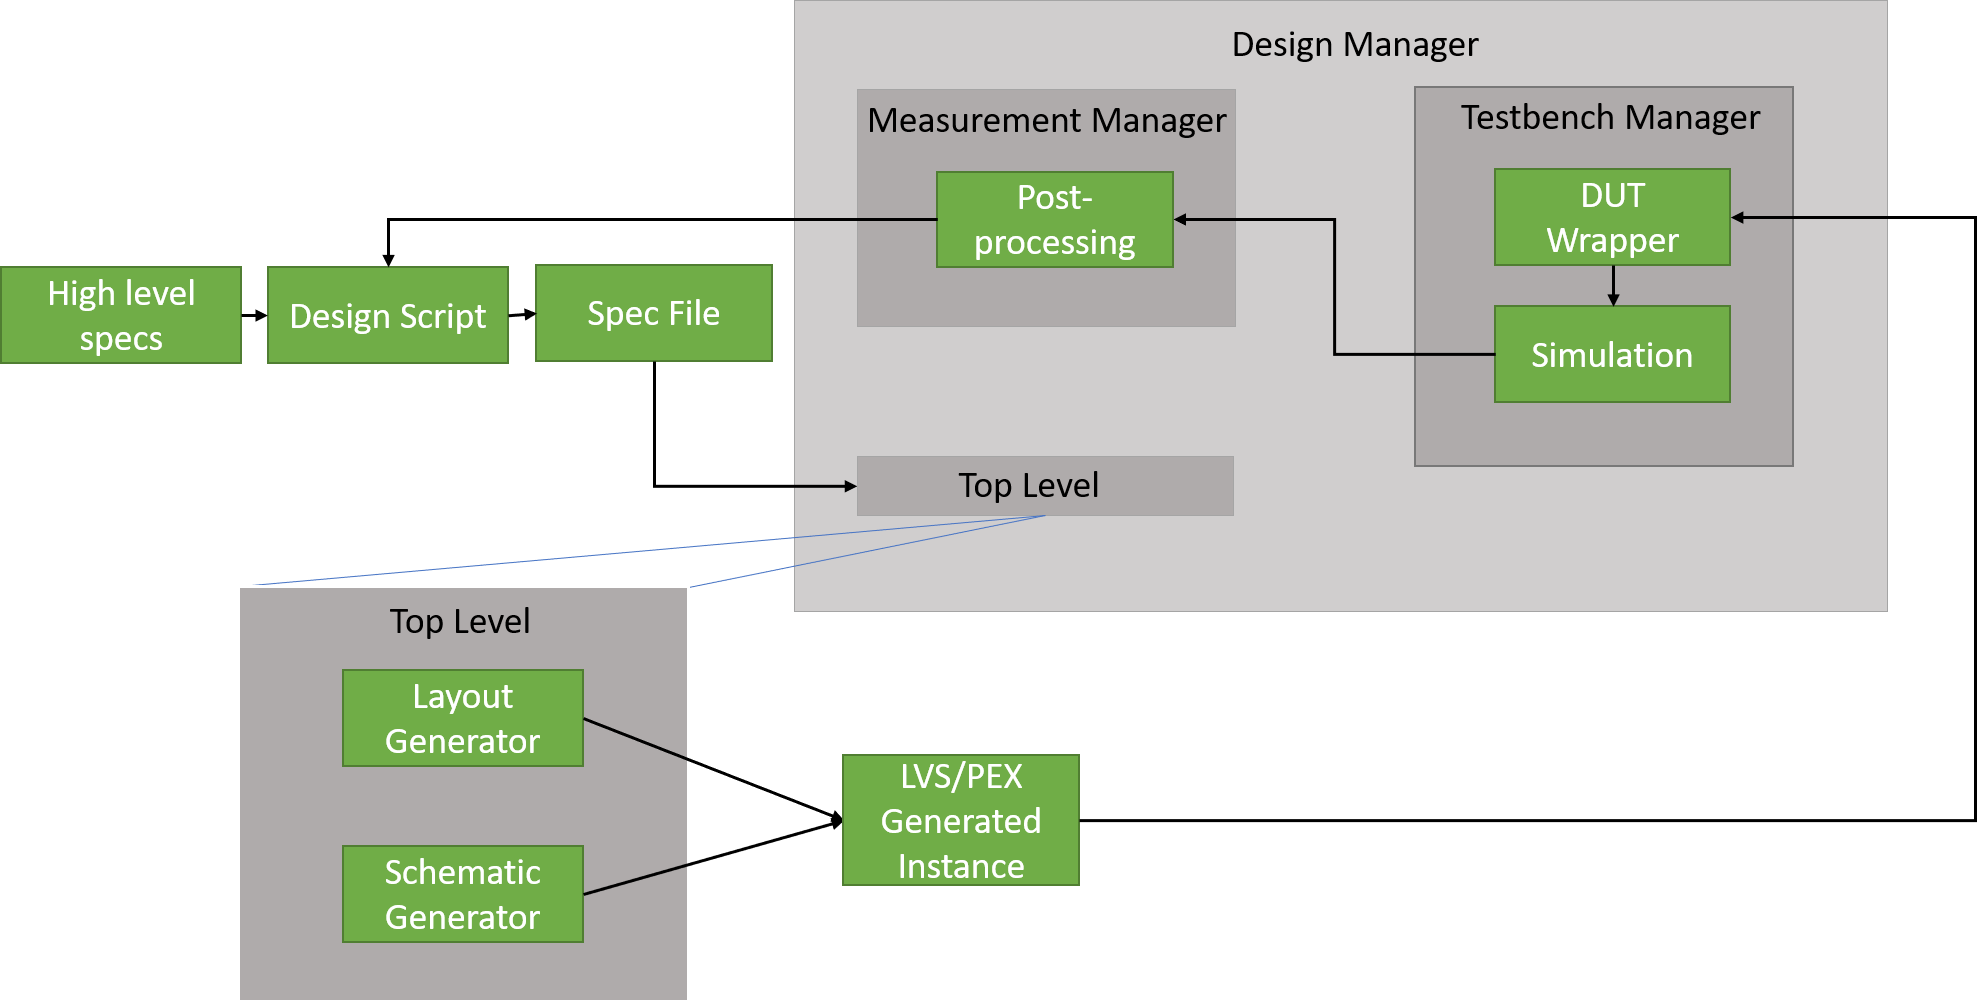
\includegraphics[width=0.8\textwidth]{bag_overview}
\caption{BAG Overview}
\label{fig:bag_top_level}
\end{figure}
As discussed in [CITATION HERE], BAG is a framework that allows users to create, use and test process portable analog generators. Designers can create template schematics and write a scripted layout generator that incorporates their design methodology in a process-portable, parametrized way. At the highest level, the user inputs parameters such as device dimensions and passive values into a specification file, and a script will generate a schematic, LVS tested layout and a PEX netlist. The main advantage is that the design loop discussed in chapter 1 is significantly reduced in size as post-layout effects can be directly included into the flow. 

As will be discussed in later sections, there are a few main components to a ``complete" generator. At the lowest levels are the layout generator and schematic generator. These are responsible for the physical process of generating the circuit representation and layout. In order to use these, there is also a top level script who's responsibility is to read a parameters file and run the schematic/layout generators with these specifications. The top level is also responsible for deciding whether or not to run LVS/PEX on the generated instance.

At an even higher level is the notion of a design script and design managers. Design manager is a class responsible for using the top level generator mentioned previously and overseeing the process of running tests and post-processing on test results. Design manager has associated testbench scripts which are responsible for connecting the generated device into a previously made test harness. The testbench script maps the pins of the instance to the pins of the test harness and runs predetermined SPICE simulations (i.e. AC, transient, S-parameters) before exporting the results to Python. Design manager can then pass the results to a measurement manager which can process, plot, etc. The entire process can be visualized as in \ref{fig:bag_top_level}.

The notion of a design script is an even higher level concept which allows a designer to encode their design procedure automatically into a close-looped script. The user can write a script that computes passive and transistor sizings, allow design manager to generate and test the post-PEX netlist, and iterate based on the results. The possibility of incorporating a design script will be discussed later, although a design script is not presented in this work. Design scripts are discussed in further detail in [CITATION HERE, ERIC AND KOUROSH].
%\begin{figure}\centering
%\parbox{.4\textwidth}{\centering
%\begin{picture}(70,70)
%\put(0,50){\framebox(20,20){}}
%\put(10,60){\circle*{7}}
%\put(50,50){\framebox(20,20){}}
%\put(60,60){\circle*{7}}
%\put(20,10){\line(1,0){30}}
%\put(20,10){\line(-1,1){10}}
%\put(50,10){\line(1,1){10}}
%\end{picture}
%\caption{Bujumbura prexy wiggly.}}
%\hfill
%\parbox{.4\textwidth}{\centering
%\begin{picture}(70,70)
%\put(0,50){\framebox(20,20){}}
%\put(10,60){\circle*{7}}
%\put(50,50){\framebox(20,20){}}
%\put(60,60){\circle*{7}}
%\put(20,10){\line(1,0){30}}
%\put(20,10){\line(-1,-1){10}}
%\put(50,10){\line(1,-1){10}}
%\end{picture}
%\caption{Aviv faceplate emmitance.}}
%\end{figure}

\section{Layout Generators}
Layout generators are arguably the most important portion of the process and are extensively discussed in [CITATION HERE, ERIC]. BAG offers a set of functions for drawing transistors, automatically routing metals, drawing vias, etc. to allow the same capability that hand design would produce. The goal of the designer is to use these functions in a generic way that automatically computes where and how to draw connections that will be DRC and LVS clean regardless of the input specifications. 

The typical process of generating a large complex block is to start with small cells, like an inverter or an active diff amp using AnalogBase. AnalogBase is a class in BAG used for drawing layouts comprised entirely of transistors. Firstly, the user draws a schematic template, like shown in \ref{fig:sch_templ}.
\begin{figure}[h]
\centering
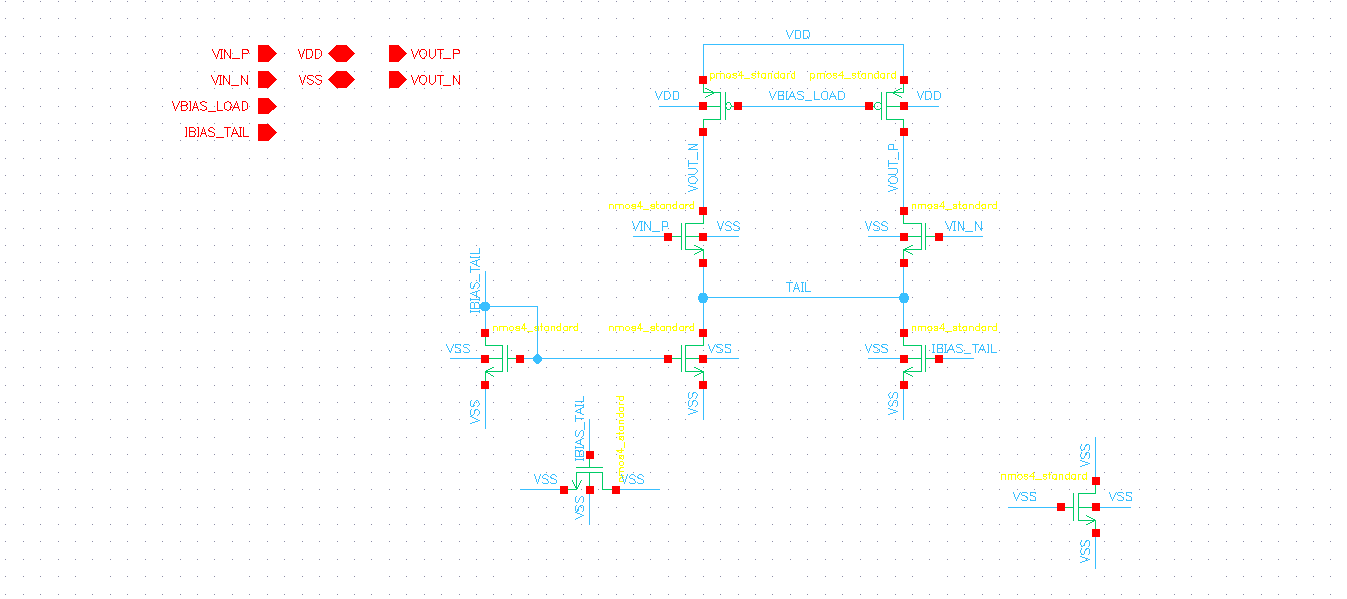
\includegraphics[width=0.8\textwidth]{sch_temp}
\caption{Schematic Template Example}
\label{fig:sch_templ}
\end{figure}
This template holds only a human-readable description of the connections. The schematic will be copied over with actual values filled in by BAG afterward. One thing to note is the presence of seemingly useless transistors, like in the bottom right. These transistors are used by BAG to properly create dummy transistors in the layout, and anything else can be removed if not used in the schematic generator. Using the schematic template, the user then decides how many rows of transisters will be in the layout, and assigns a number of transistors to each row. BAG will then draw the all of the required polygons for the metal connections to the MOS devices, transistors and everything else. An example base layout with no wiring done of the schematic in \ref{fig:sch_templ} is shown in \ref{fig:base_layout_metal}.
\begin{figure}[h]
\centering
\begin{subfigure}{.4\linewidth}
  \centering
  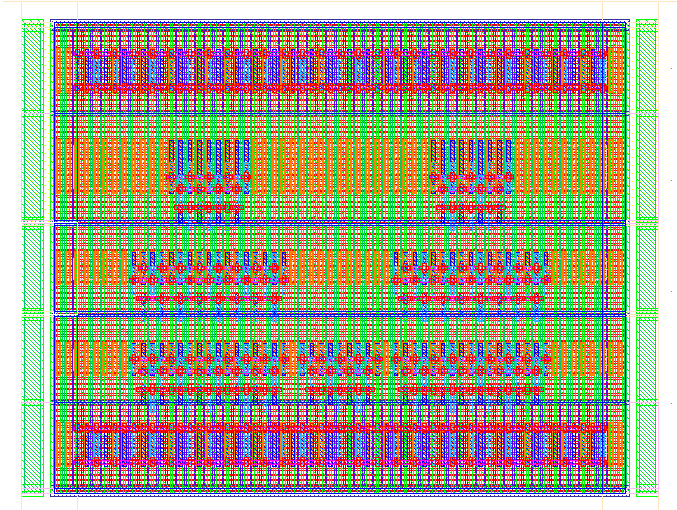
\includegraphics[width=\textwidth]{base_full}
  \caption{Base layout of transistors with active regions, poly, etc.}
  \label{fig:sfig1}
\end{subfigure}
\begin{subfigure}{.4\linewidth}
  \centering
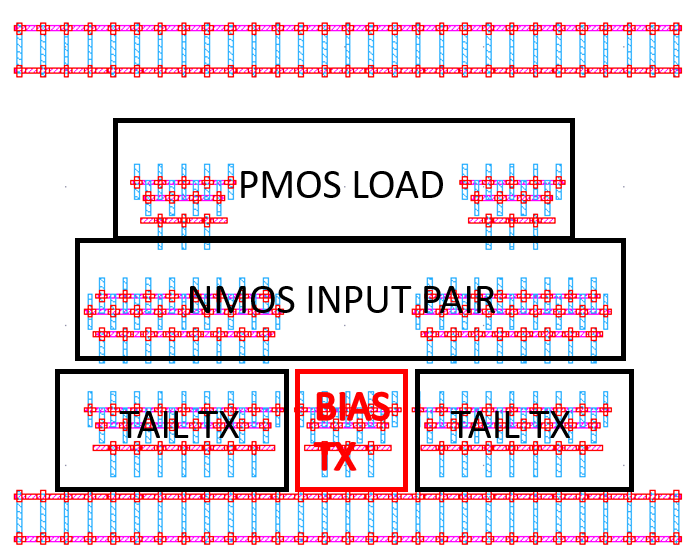
\includegraphics[width=0.9\textwidth]{base_metal_annotated}
  \caption{The same layout with only metal connection layers shown. Annotated with locations of transistors.}
  \label{fig:sfig2}
\end{subfigure}
\caption{Base layout}
\label{fig:base_layout_metal}
\end{figure}
\clearpage
After drawing the base layout, users can then specify how to connect wires and ports by specifying a metal layer, a wire width and a track. Tracks are an invisible grid that spans the design space used by BAG to place wires properly. \ref{fig:base_with_wires} shows the connections made by BAG.
\begin{figure}[h]
\centering
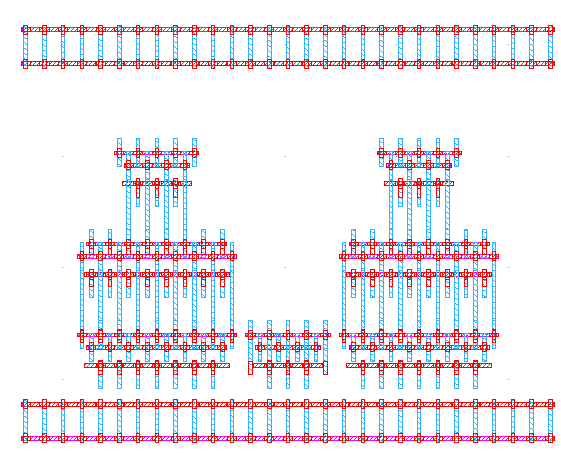
\includegraphics[width=0.6\textwidth]{base_metal_conns}
\caption{Transistor Wiring}
\label{fig:base_with_wires}
\end{figure}
Lastly, the user finalizes connections and adds pins to wires. In the final step, BAG will draw dummy transistors and create straps for the power supplies, automatically routing the dummies connections to the supply, like in \ref{fig:finished_layout}.
\begin{figure}[h]
\centering
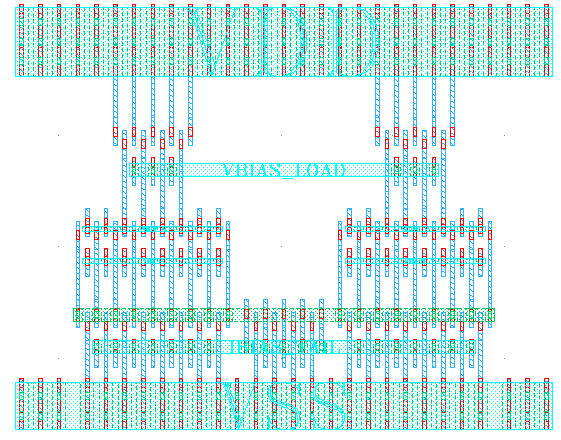
\includegraphics[width=0.6\textwidth]{full_layout}
\caption{Finished Layout}
\label{fig:finished_layout}
\end{figure}
With a finished layout generator, the user can now arbitrarily change their transistor specifications which will be reflected automatically in the wiring and sizing. \ref{fig:width_changes} shows the same generator with various width and number of finger choices.
\begin{figure}[h]
\centering
\begin{subfigure}{.4\linewidth}
  \centering
  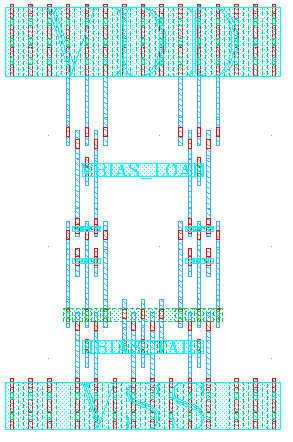
\includegraphics[width=0.6\textwidth]{small_width}
  \caption{}
  \label{fig:sfig1}
\end{subfigure}
\begin{subfigure}{.4\linewidth}
  \centering
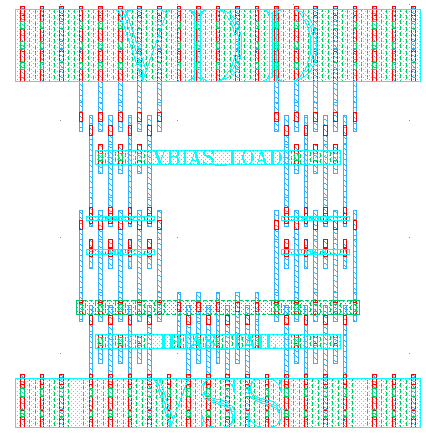
\includegraphics[width=0.6\textwidth]{med_width}
  \caption{}
  \label{fig:sfig2}
\end{subfigure}
\begin{subfigure}{.4\linewidth}
  \centering
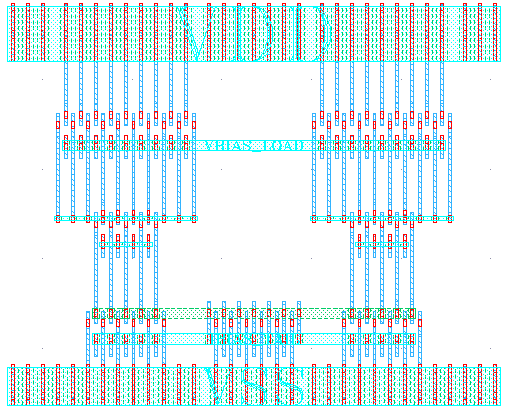
\includegraphics[width=0.6\textwidth]{large_width}
  \caption{}
  \label{fig:sfig2}
\end{subfigure}
\caption{Differential amplifier layout with various widths and number of finger choices.}
\label{fig:width_changes}
\end{figure}
\clearpage
BAG also offers heriarchy in layout using TemplateBase [CITATION HERE, ERIC]. When a library of smaller cells are created, the user can then ``stamp" these cells into a larger unit and connect them together to form more complex systems. An example of a circuit containing a differential TIA and a CTLE is shown in \ref{fig:tia_ctle}.
\begin{figure}[h]
\centering
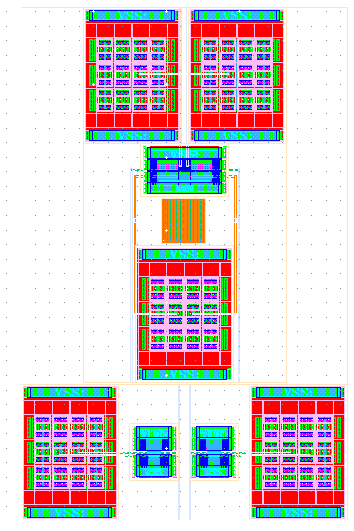
\includegraphics[width=0.2\textwidth]{tia_ctle}
\caption{Differential TIA and CTLE}
\label{fig:tia_ctle}
\end{figure}
The benefit of codifying the layout procedure is that configuration can be automatically included. For example, should a designer want variable resitors in their circuit, they may opt for a resistor DAC. Resistor DACs are often an arbitrary number of arrayed unit resistors with digitally controlled switches. Using TemplateBase, we can place any amount of template layouts which allows for a single generator with a large degree of freedom. The user can choose how many bits, what type of switch to use (NMOS, PMOS, passgate), and even whether or not to include local inversion for the passgate. An example of multiple resistor DAC layouts are shown in \ref{fig:dac}.
\begin{figure}[h]
\centering
\begin{subfigure}{.4\linewidth}
  \centering
  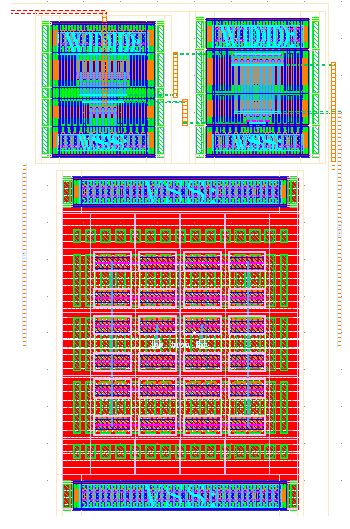
\includegraphics[width=0.2\textwidth]{res_dac_1}
  \caption{1 bit}
  \label{fig:sfig1}
\end{subfigure}
\begin{subfigure}{.4\linewidth}
  \centering
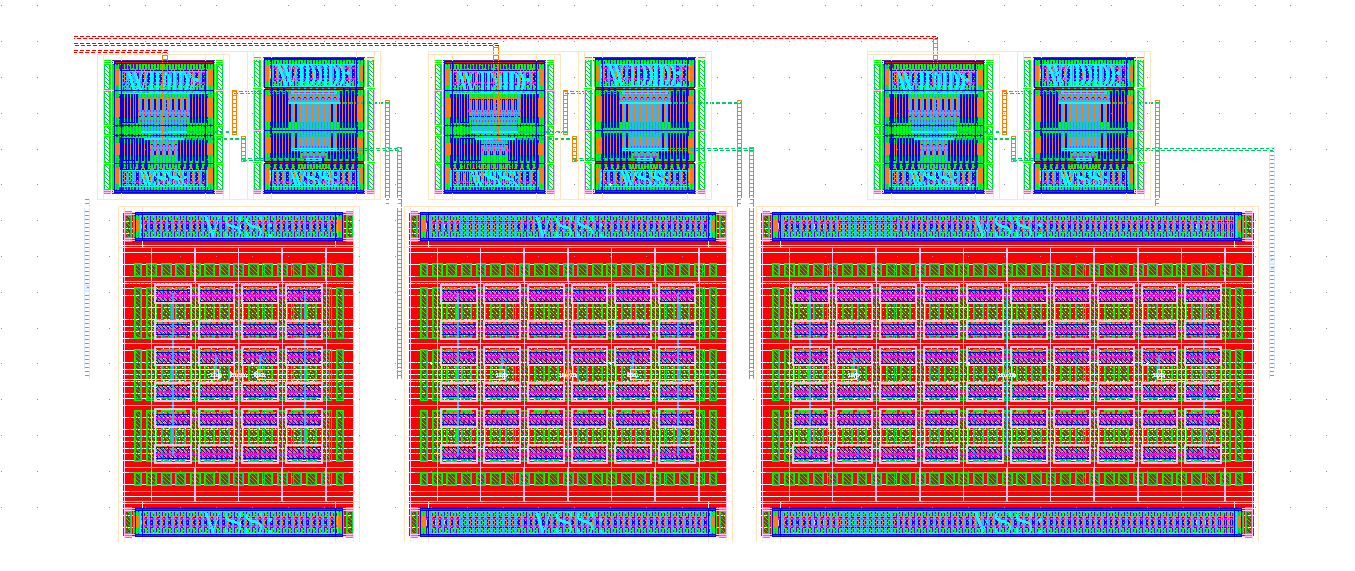
\includegraphics[width=1\textwidth]{res_dac_3}
  \caption{3 bits}
  \label{fig:sfig2}
\end{subfigure}
\begin{subfigure}{.5\linewidth}
  \centering
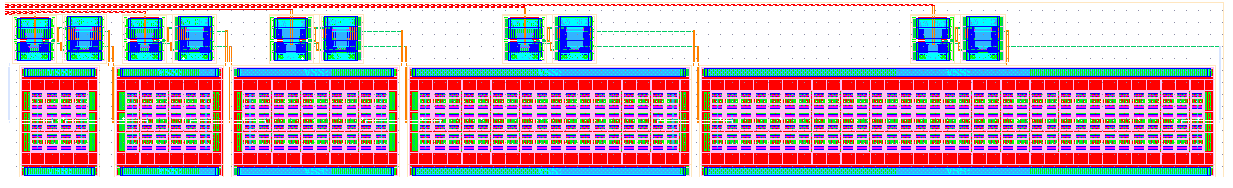
\includegraphics[width=1.2\textwidth]{res_dac_5}
  \caption{5 bits}
  \label{fig:sfig2}
\end{subfigure}
\caption{Various resistor DAC layouts}
\label{fig:dac}
\end{figure}
\clearpage
\section{Schematic Generators}
Schematic generators control the process of copying the template schematic mentioned previously and assigning values to the components based on the inputted spec file [CITATION HERE, ERIC]. These generators have the capability of arraying and deleting instances, removing, adding or renaming pins and other simple operations.

Generally the user simply inputs commands to pass the component values into the design; but for circuits such as the resistor DAC in the previous section, the user can automatically array and resize components based on the layout like shown in \ref{fig:resdac_sch}. 
\begin{figure}[h]
\centering
\begin{subfigure}{.5\linewidth}
  \centering
  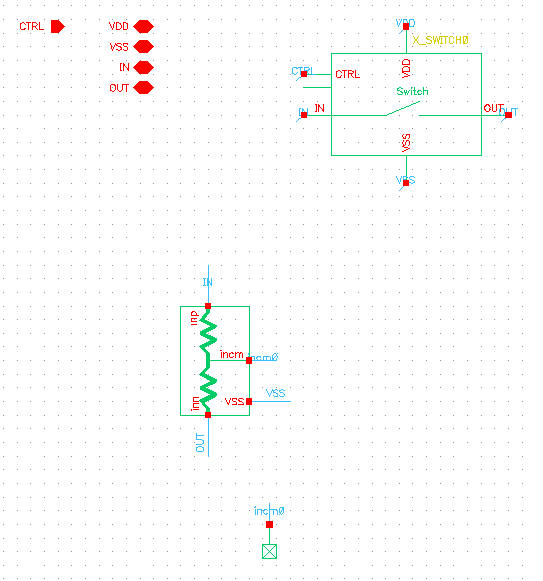
\includegraphics[width=\textwidth]{res_dac_1_sch}
  \caption{1 bit}
  \label{fig:sfig1}
\end{subfigure}
\begin{subfigure}{0.6\linewidth}
  \centering
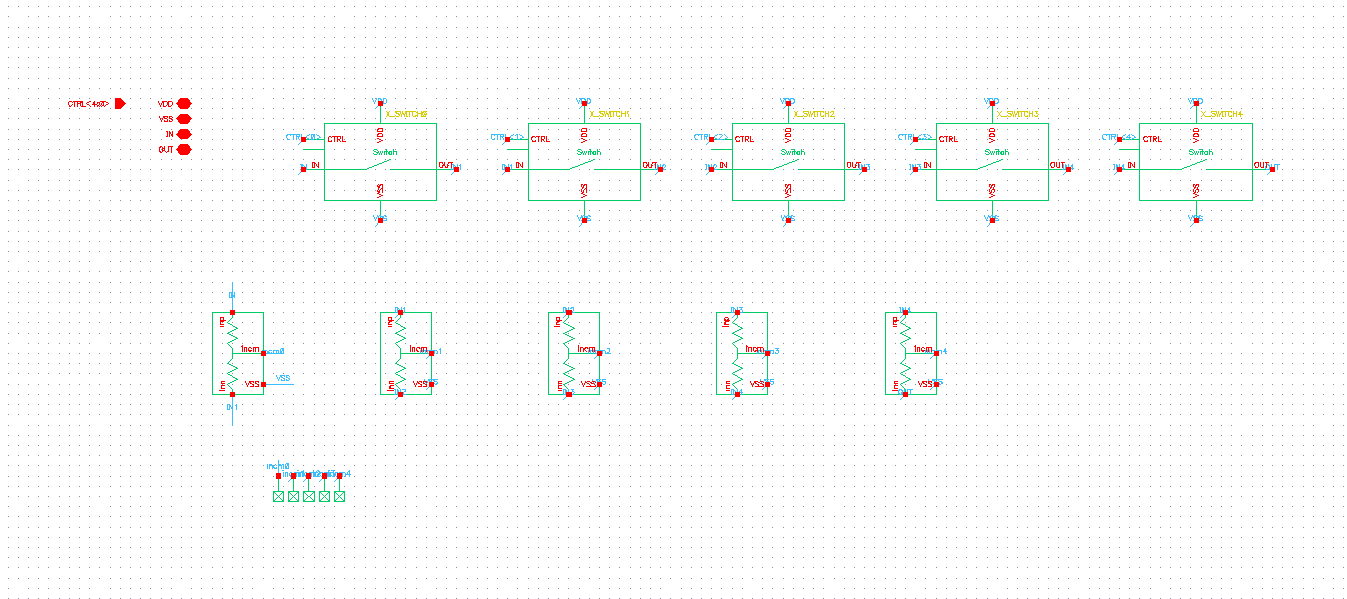
\includegraphics[width=\textwidth]{res_dac_5_sch}
  \caption{5 bits}
  \label{fig:sfig2}
\end{subfigure}
\caption{Various resistor DAC layouts}
\label{fig:resdac_sch}
\end{figure}
\clearpage
\section{Design Manager and Testbenches}
As shown in \ref{fig:bag_top_level}, design manager is a separate entity to that of the layout and schematic generators [CITATION HERE, ERIC]. Design managers contain within them multiple testbench managers that each have their own corresponding measurement manager. In the specifications file, the user decides which tests to run and design manager will generate an instance and pass it through the chosen simulations. This is the method used to test the circuits described in Chapter 4. 

Tests are made by the user in a similar method to schematic generators. The user specifies a testbench setup with a generic DUT block and adds input sources and pins. Within a specifications file, the user describes how to wrap the inputs of the DUT to the generic block, as well as what outputs to save. These outputs are sent to the measurement manager where the user can, for example, compute 3dB frequencies, DC gain, etc. and save the results if desired. Multiple testbenches can be run in one instance.

An example testbench manager, \texttt{generic\_AC\_TB},\footnote{This testbench, and all others used in this report come courtesy of Kourosh H. of team Vlada.} inputs an AC voltage or current and runs an AC simulation and noise simulation. The corresponding measurement manager sifts through the data and (regardless of the transfer function shape) computes the DC gain and overall bandwidth. The noise data is integrated and reported, as well as CMRR. 